% N.B. one {latexonly} environment commented out so that its
% contents can be displayed in the HTML version of this template.
% Uncomment it for actual use!
%
% Use text editor to replace:
%
%       author   --- author's login name
%       thisdoc  --- document filename (as in thisdoc.tex, thisdoc.ps)
%       psiz     --- size of compressed PostScript file
%
%       Document_Date          --- current date
%       Document_Short_Title   --- header text for Postscript
%       Document_Long_Title    --- full document title
%       Author_Name            --- full author name
%       Author_City            --- Charlottesville, Socorro, etc.
%       Author_State           --- Virginia, New Mexico, etc.
%
%       (non-NRAO: also replace institute name/acronym and country?)
%

\documentclass{article}
\usepackage{html,makeidx,epsf}
\usepackage{graphicx}
\usepackage{amssymb}
\usepackage{amsmath}
%%\usepackage{media9}
\usepackage[overload]{empheq}

%\renewcommand{\bibname}{References}

%
% Add home page navigation button -- edit the URL!
%


\htmladdtonavigation{\htmladdnormallink
  {\htmladdimg{jetscalecropped.png}}{cv.pdf}}

%
% define hyperlink URLs:
%

\def\linkedin{https://www.linkedin.com/in/ilari-angervuori-0a1358160/}
\def\soundcloud{https://soundcloud.com/ilari-angervuori}
\def\github{https://github.com/Rugiero}
\def\pass{https://www.passwordstore.org/}
%%\def\cv{https://www.dropbox.com/s/jem3l3jabcyex9s/Curriculum_Vitae_Ilari_Angervuori.pdf?dl=0}
\def\cv{cv.pdf}
\def\academiccv{acv.pdf}
\def\hal{https://hal.inria.fr/inria-00403039v1/}
\def\hall{https://hal.inria.fr/inria-00403040v4/document}
\def\ray{https://en.wikipedia.org/wiki/Rayleigh_fading}
\def\ric{https://en.wikipedia.org/wiki/Rician_fading}
\def\gaus{https://en.wikipedia.org/wiki/Gaussian_noise}
\makeindex

\begin{document}

%
%  Page formatting for Postscript output
%

\title{
  {\bf A glimpse to my mind}
}

\author
    {
      Ilari Angervuori\\
    }

    \date
        {
          {Last update 11.05.2022}\\
        }

        \begin{center}
          \htmladdnormallink{Linkedin}{\linkedin}\\
          \htmladdnormallink{Soundcloud}{\soundcloud}\\
          \htmladdnormallink{GitHub}{\github} \\
          \htmladdnormallink{CV}{\academiccv}\\
        \end{center}

        %\begin{latexonly}
        %\markright{Document_Short_Title}
        \maketitle
        % uncomment to run:
        %\end{latexonly}

        \tableofcontents

        \pagebreak
        \section{About me}


        
                I am a Finnish mathematician interested in engineering. Read about my life, or jump straight to my professional records in the subsections below. Also, check out my blog.

                \parbox{\textwidth} {
        I graduated in 2009 from Munkkiniemi high school. Mathematics was a subject I had naturally thrived in -- so, after some bumps and turns,  I found myself in the University of Helsinki studying mathematics. And yeah, indeed, I love mathematics -- I love the apparent universality of it. This subject is without a doubt debatable, but, at least in some sense, I like to think that mathematical truths are universal in the truest sense of the word; they are eternal, they are the same everywhere, regardless of the physical universe we live in. Alien in another galaxy will end up in the same mathematical truths we do. Alien in another universe will end up in the same mathematical truths we do. Mathematics has the power to explain what we see in our everyday life. Mathematics is not only natural science but a form of art and poetry. Mathematics is music -- music is mathematics.

        While studying mathematics, physics and computer science, I took some courses on economics. That inspired me to write my Bachelors thesis on optimal control theory. I worked on the problem of how increasing public investments affect the GDP. I did not find any breakthrough, but it was an intriguing subject.

        I proceeded with my graduate studies studying applied mathematics. I studied subjects like partial differential equations, functional analysis, dynamical systems, and  -- the University of Helsinki's proudness -- complex analysis. (My thesis advisor said that, in a moral sense, you cannot graduate from the University of Helsinki without taking some courses on Complex analysis, because a lot of the discipline has been developed in the university.) In addition, as a more ``practical'' subject, I studied some inverse problems. Summa summarum, I studied a wide range of fields in mathematics.

        During my graduate studies, I spent half a year in Utrecht, Netherlands, studying more applied analysis of varying subjects (searching periodic orbits in the Lorentz attractor as an example of a course -- that I failed). At Utrecht University, I got the inspiration for a subject for my future master's thesis; the Finite Element Method. After I got back to Helsinki from the exchange, I had a chance to study more about the finite element method in Aalto University's courses. (Aalto University is a consortium of the Helsinki University of Technology, the Helsinki School of Economics and the University of Art and Design Helsinki.) While writing my thesis I also taught basic mathematics courses at the University of Helsinki and gained valuable experience in the pedagogical area.

        In the binge of graduation, I started to look for future opportunities. I looked for coding jobs in Helsinki and Tallinn, jobs for mathematicians in the mapping industry, continuing at some university to pursue a PhD etc. I ended up in the last one as doors opened for me into Aalto University's Department of Signal Processing and Acoustics to research low earth orbit satellite communications.

        My professional ambitions are in improving the lives of people globally. Communications play an essential in the picture. (But contain some challenging problems also, as we have seen with the social media.) Through effective communication, we can share knowledge, control resources, discuss issues etc. -- however, globally, the communication infrastructure is still not nearly complete. My interests contain, but are not limited to, communications, particularly wireless networks and signal processing. My dream is to share my knowledge in the process towards a free and honest world. (Pardon me for the cliches.)
        
        }
        %% One milestone in my way to engineering started at 2009, thee year of my high school graduation, when I got in to study Electrical engineering in the Helsinki University of technology (TKK). Mathematical disclipline was a natural choice for me as during my highschool years in Helsinki, Munkkinimemi, mathematics and physics where areas where I could get by well without too much effort – or the effort did not feel overwhelmingly bad because I was genuinely interested in these arts. Vastness of space and mathematical poet-like ability to describe the world has always fascinated me – there is something calmfull in chewing the formulas and gradually starting to grasp the mathematical description by your own intuition.

        %% The first year in TKK went by. How ever much I loved engineering, I loved partying equally much. Couple of semesters went without any credits and one day I decided that electrical circuits is not for me -- I wanted to lean towards natural sciences, maybe to Meteorology, or Geophysics. Anyways, at that momement I was not into technology and I did not feel home in University of technology.  So after one year studying in TKK and one -- admittedly interesting -- year in the service of the Finnish Defence Forces I started to study physics in the University of Helsinki.

        %% I started my freshman year with meteorologists. First year was for most part studying in basic physics courses and mathematics as a minor subject. I made some ever lasting friendships during the period with meteorologists, but I never completed one course in meteorology. I was more into physics and mathematics. In the end the minor subject turned to be my major interest, and I changed my major to mathematics. I suppose I had more or less kind of artistic mind set and thought that mathematics grasps the heart of reality in a more rudimentary manner than physics. It is the universal language – I mean – so universal that it does not depend on our universe; the prime numbers are there regardless of what ever value the gravitational constant happens to be. So I started to study real analysis, complex analysis, topology, functional analysis in the department of mathematics in the University of Helsinki. My goal was to pursue a master degree in Applied Analysis.




        

        \begin{figure}
          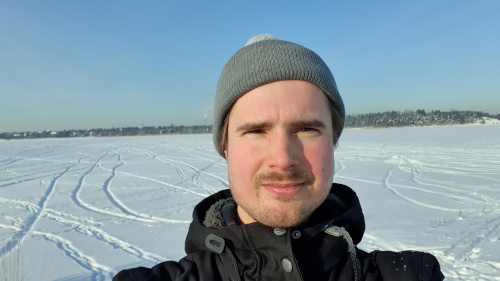
\includegraphics[width=\linewidth]{me1.jpg}
          \caption{Me in my beloved home town Helsinki in the middle of the summer (well, technically I am in Espoo, Otaniemi – and it is a snowy and shiny day in February, frozen sea seen in the background)}
        \end{figure}

        
        I am keeping up a monthly blog that you can find in the blog posts section. It handles stuff encountered in my daily professional life (and I keep the right to write about other subjects). I hope you will find it interesting. 
        
        Btw, In the free time I love music, literature, long walks listening to podcasts, coffee and beer.

        \subsection{Education}
        \begin{itemize}
        \item 2016 Bachelor of Science University of Helsinki\\
        \item 2018 \htmladdnormallink{Master of Philosophy}{https://helda.helsinki.fi/handle/10138/273474} University of Helsinki
        \end{itemize}

        
        
        \subsection{Publications}
        

        \begin{itemize}
        \item
          Ilari Angervuori and  Risto Wichman, ``A Closed-Form Approximation of the SIR
          Distribution in a LEO Uplink Channel'', GLOBECOM 2022, Rio de Janeiro, Brazil, submitted for publication.
          
        \item
         Ilari Angervuori,  Niloofar Okati, Taneli Riihonen,  Risto Wichman, ``Uplink Interference Characterization and Coverage Analysis of Modern {LEO} and {VLEO} Networks: A Stochastic Geometry Approach'', IEEE Transactions on Communications, submitted for publication.
                  
        \item 
          Okati, N., Riihonen, T., Korpi, D., Angervuori, I. Wichman, R., Aug 2020, ``Down-link Coverage and Rate Analysis of Low Earth Orbit Satellite Constellations Using Stochastic Geometry'',  IEEE Transactions on Communications. 68, 8, p. 5120-5134 9079921.\\
          
        \item A. Yastrebova et al., ``Theoretical and Simulation-based Analysis of Terrestrial Interference to LEO Satellite Uplinks,'' GLOBECOM 2020 - 2020 IEEE Global Communications Conference, Taipei, Taiwan, 2020, pp. 1-6, doi: 10.1109/GLOBECOM42002.2020.9347980.
          
        \item Niloofar Okati, Islam Tanash, Taneli Riihonen, Ilari Angervuori, Wichman Risto, ``Performance Evaluation of Low Earth Orbit Communication Satellites'', 2019
          
        \item Ilari Angervuori, Wichman Risto, Niloofar Okati, Taneli Riihonen, ``On routing protocols in inter-satellite communications'', 2019
                    
        \end{itemize}


        \section{Blog posts 2021}
        General thoughts on mathematics and engineering, practical instructions, artistic non-sense. The themes of this blog are much inspired by the challenges encountered in my professional life.

        \subsection{January – Poisson Process on a Sphere}
        \htmladdnormallink{Poisson point process}{https://en.wikipedia.org/wiki/Poisson_point_process} can be generalized to general \htmladdnormallink{manifolds}{https://en.wikipedia.org/wiki/Manifold}. Particularly, Poisson process on a three dimensional sphere surface is useful. Nicely enough, Poisson process on a unit sphere is equivalent to process in a two dimensional area $ A = [-\pi,\pi] \times [-1,1]$ through the area preserving mapping from $A$ to geographical coordinates
        \begin{equation}
          (x,y) \mapsto (1,x,\sin^{-1}(y)) \nonumber.
        \end{equation}


        Resulting process interpreted in geographical coordinates $(r,\theta,\varphi)$ is a Poisson point process on a sphere of radius $r$.  Following codes returns a scatter plot of Poisson points on the unit sphere.



        GNU Octave or Matlab:
\begin{verbatim}
%Plot random points on a unit sphere. Returns the points in a vector ref in cartesian coordinates
function refc = poissononsphere(density)
  yMin = -1; yMax = 1;
  xMin = -pi; xMax = pi;
  
  xDelta = xMax - xMin; yDelta = yMax - yMin; %Rectangle dimensions
  numbPoints = poissrnd(density);    %Number of points in the area is a Poisson variable of intensity given as density
  x = xDelta*(rand(numbPoints,1)) + xMin;    %Pick points from uniform distribution
  y = yDelta*(rand(numbPoints,1)) + yMin;    %Map referencepoints to geographical coordinates
  ref = [x y]';

  refs = [x'; asin(y)'];%Map geographical coordinates to Cartesian coordinates on a unit circle
  r = 1;
  refc = [r*sin(refs(2,:)+pi/2).*cos(refs(1,:)+pi);...
          r*sin(refs(2,:)+pi/2).*sin(refs(1,:)+pi);...
          r*cos(refs(2,:)+pi/2)];

  figure(1)    %Plot
  [X, Y, Z] = sphere;
  surf(X,Y,Z,'EdgeColor','none','FaceColor','black');
  hold on
  scatter3(refc(1,:),refc(2,:),refc(3,:),10,...
           'MarkerFaceColor','yellow',...
           'MarkerEdgeColor','red');
  axis equal
end
\end{verbatim}

Python:

\begin{verbatim}
import numpy as np
import scipy.stats
import matplotlib.pyplot as plt
from mpl_toolkits.mplot3d import axes3d

#Rectangle dimension
xMin = -np.pi; xMax = np.pi;
yMin = -1; yMax = 1;
xDelta = xMax - xMin; yDelta = yMax - yMin; #rectangle dimensions

#Density parameter of the Poisson point process. Mean number of points on the sphere
lambda0=1000; 

#Simulate Poisson point process

#Number of point in the area is a Poisson variable of intensity lambda0
numbPoints = scipy.stats.poisson( lambda0 ).rvs()
x = xDelta*scipy.stats.uniform.rvs(0,1,((numbPoints,1)))+xMin
y = yDelta*scipy.stats.uniform.rvs(0,1,((numbPoints,1)))+yMin

#Transform to geographical coordinates
x = x
y = np.arcsin(y)
#Plotting
fig = plt.figure()
ax = plt.axes(projection="3d")
ax.scatter(np.sin(y+np.pi/2)*np.cos(x+np.pi),np.sin(y+np.pi/2)*np.sin(x+np.pi),np.cos(y+np.pi/2), color='r' )
plt.show()

\end{verbatim}

Wolfram Language:
\begin{verbatim}
(*lambda is the mean number of points on the unit sphere*) 
  poissononsphere[lambda_] := 
  Module[{nrofpoints, phi, theta, radius, refc, polarp}, 
   nrofpoints = RandomVariate[PoissonDistribution[lambda]];
   polarp = 
    Table[{RandomVariate[UniformDistribution[{-Pi, Pi}]], 
      ArcSin[RandomVariate[UniformDistribution[{-1, 1}]]]}, 
     nrofpoints];
   radius = 1;
   refc = 
    Table[{radius*Sin[polarp[[i]][[2]] + Pi/2]*
       Cos[polarp[[i]][[1]] + Pi],
      radius*Sin[polarp[[i]][[2]] + Pi/2]*Sin[polarp[[i]][[1]] + Pi],
      radius*Cos[polarp[[i]][[2]] + Pi/2]}, {i, nrofpoints}];
   refc
   ];
   ListPointPlot3D[poissononsphere[500], BoxRatios -> {1, 1, 1}]  
\end{verbatim}

\begin{figure}
  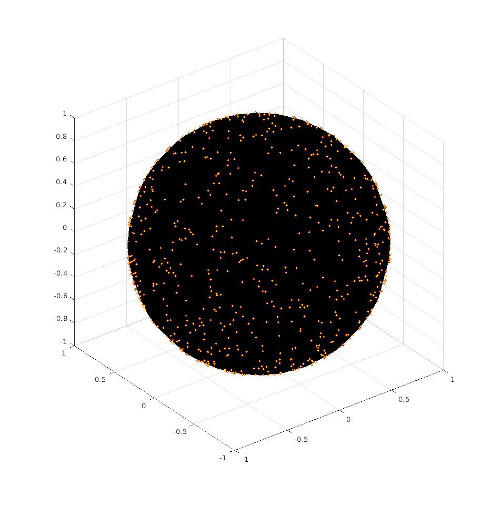
\includegraphics[width=\linewidth]{poissononsphere.jpg}
  \caption{Are the stars Poisson distributed in the sky?}
\end{figure}

\begin{figure}
  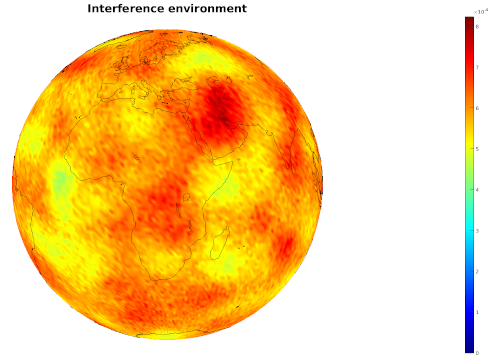
\includegraphics[width=\linewidth]{interferenceenvironment.png}
  \caption{Aggregate interference power in a satellite receiver represented by a color – interfering sources are considered to be Poisson distributed on Earth}
\end{figure}

References:
\begin{itemize}
\item D. J. Daley and D. Vere-Jones, The General Poisson Process in  ``An introduction to the theory of point processes''. New York: Springer, 2003, pp. 39. 
\item Stoyan, Dietrich. et al. ``Stochastic Geometry and Its Applications''. 3rd ed. Chichester: Wiley, 2013. Print.
\item  \htmladdnormallink{H. Paul Keeler's Blog}{https://hpaulkeeler.com/simulating-a-poisson-point-process-on-a-sphere}
\end{itemize}




\subsection{February – Controlling Your Passwords with Pass}
Pass is a nice Unix style free and open source wallet for keeping your passwords safe. Here is a brief look how to set it up in Ubuntu.

\begin{itemize}
\item Install the application in the terminal \\
\begin{verbatim}
sudo apt install pass  
\end{verbatim}
\item Check for existing GPG keys \\
\begin{verbatim}
gpg --list-keys 
\end{verbatim}
\item If no keys were found generate a key pair \\
\begin{verbatim}
gpg --generate-key
\end{verbatim}
\item Copy the name of the key and initialize pass\\
\begin{verbatim}
pass init ABCDEFGHIJKLMNOPQRSTUV1234, 
\end{verbatim}
where ABCDEFGHIJKLMNOPQRSTUV1234 is the name of the key.
\item Generate a password with \\
\begin{verbatim}
pass generate keyfolder/newkey 
\end{verbatim}
List passwords
\begin{verbatim}
pass
\end{verbatim}
Copy a password to clipboard \\
\begin{verbatim}
pass keyfolder/newkey -c
\end{verbatim}
For more commands
\begin{verbatim}
man pass
\end{verbatim}
\end{itemize}

Connect pass to git so it is easy to keep track of changes with multiple machines.

\begin{itemize}
\item Export your public and private key to a file with \\
\begin{verbatim}
  gpg --export --output public.key ABCDEFGHIJKLMNOPQRSTUV1234 
  gpg --export-secret-key --output private.key ABCDEFGHIJKLMNOPQRSTUV1234,
\end{verbatim}
where ABCDEFGHIJKLMNOPQRSTUV1234 is your key name.\\
\item Now we can initialize the git repository with these keys. Move public.key and private.key through a safe channel to a computer you wish to use pass in. Import the keys to the machine \\
\begin{verbatim}
gpg --import public.key
gpg --import private.key
\end{verbatim}
\item After importing keys to a new machine you can initialize pass
\begin{verbatim}
pass init ABCDEFGHIJKLMNOPQRSTUV1234
\end{verbatim}

\item Initialize your git repository. Make a new repository named pass-store e.g. to GitHub if you are doing this first time before the following commands\\
\begin{verbatim}
pass git init 
pass git remote add origin git@repo.com:myname/pass-store
 \end{verbatim}
\item Get password data from the server (from a non-empty repository, otherwise skip)
\begin{verbatim}
pass git pull origin master --allow-unrelated-histories
pass git commit -am "firstcommit"
\end{verbatim}
\item Do some changes and pass will automatically commit them. Push and set upstream \\
\begin{verbatim}
pass git push --set-upstream origin master 
\end{verbatim}
\item From here on you can use the familiar git commands \\
\begin{verbatim}
pass git pull 
pass git push 
\end{verbatim}
\end{itemize}
Stay safe :)


References:

\begin{itemize}
\item \htmladdnormallink{Password Store}{\pass}
\end{itemize}


\subsection{March – Signal Propagation in a City}
Mobile telephone signal propagation in a city is characterized essentially by obstacles, such as buildings and cars, that \htmladdnormallink{attenuates}{https://en.wikipedia.org/wiki/Attenuation}, \htmladdnormallink{reflects}{https://en.wikipedia.org/wiki/Reflection_(physics)}, \htmladdnormallink{refracts}{https://en.wikipedia.org/wiki/Reflection_(physics)} and \htmladdnormallink{diffracts}{https://en.wikipedia.org/wiki/Diffraction} the signal. Should there be a pure line-of-sight from the transmitter to the receiver, the receiver will always receive a constant power from the transmitter conditioned that the transmitter stays at a constant distance from the receiver – this can be the case for example if you are transmitting to a near-by high base-station antenna. If there is no line-of-sight component, the signal strength will vary according to \htmladdnormallink{Rayleigh fading}{\ray} as the transmitter and/or the obstacles moves. In the case that there is only a limited line-of-sight element present, the signal strength will follow \htmladdnormallink{Rician fading}{\ric} statistics.

I animated a couple of GIFs to help us to perceive what is going on.
The first figure demonstrates how a simple sine signal propagates between buildings. You can observe how the multi-path components sum up to a signal that is amplifying in some locations and degenerating in others. You can look for both Rician conditions (lower right) and Rayleigh conditions (lower left) in the image and see how the signal behaves under those conditions. The figure was obtained by solving the Helmholtz equation by finite element method.


The second figure shows how to aggregate signal power from many mobile transmitters develops in time under Rician fading conditions. The aggregate power can be considered as interference in a receiver. You can see how the high peaks of interference power emerge at random locations. In real life, these kinds of peaks can cause decreased data rates. The figure was obtained by simulating a random walk of points in a realization of the Poisson point process on a plane.

\begin{figure}
  \includegraphics[width=\linewidth]{sin.gif}
  \caption{The white boxes represents buildings, and the little white circle is the transmitter. You can see how reflections will cause the aggregate signal strength to fluctuate by location depending on phases of the incoming reflected waves.}
\end{figure}



\begin{figure}
  \includegraphics[width=\linewidth]{rician.gif}
  \caption{Interference power field developing in time. Transmitters are Poisson distributed at random locations and moving to random directions, and the aggregate signal strength after fading is plotted. Red color represents the highest mean power of interference and deep blue represents absence of any interference. There is a line-of-sight component is present – that is, we assume  \htmladdnormallink{Rician fading}{\ric}. Red occurrences will cause remarkable disturbance in communication as interference from other transmitters gets large. Time can't be considered to be in a human perspective scale here.}
\end{figure}


References:
\begin{itemize}
\item François Baccelli, Bartlomiej Blaszczyszyn \htmladdnormallink{Stochastic Geometry and Wireless Networks, Volume I -Theory}{\hal}

\item Nicolae Cindea (2021).   \htmladdnormallink{Movie to GIF Converter}{https://www.mathworks.com/matlabcentral/fileexchange/17463-movie-to-gif-converter)}, MATLAB Central File Exchange. Retrieved June 14, 2021. 
\end{itemize}


\subsection{April – Frequentist Inference in Mathematica}

Mathematica provides a package called “Hypothesis Testing” for analyzing random data. The package includes handy objects like “Around”, representing a quantity and the uncertainty around it. The following example code returns an Around object representing the confidence interval of the estimated bias of a coin after a repeated trial. As shown in the code, the ListPlot plots Around objects as such.

\begin{verbatim}
(*Load the Hypothesis Testing Package.*)
Needs["HypothesisTesting`"];

coin[flips_, bias_] :=
 (*Make the experiment and collect the data*) 
 Module[{index, realizations, mean, conf, around},
  realizations = {};
  For[index = 1, index <= flips, index++,
   realizations =  
     Append[realizations, 
      RandomVariate[BernoulliDistribution[bias]]];
   ];
  
  (*Mean*)
  mean = Mean[realizations[[All]]];
  (*Confidence interval*)
  conf = MeanCI[realizations[[All]]];
  (*Around object*)
  around = Around[mean, Abs[conf[[1]] - conf[[2]]]]
  ]
around = coin[1000, 0.5]
ListPlot[{around}]
\end{verbatim}

References:
\begin{itemize}
\item \htmladdnormallink{reference.wolfram.com}{https://reference.wolfram.com/language/guide/HypothesisTests.html}
    
\end{itemize}


\subsection{May – Rayleigh Fading Audiolized}

When a signal is propagating through multiple paths each signal component in each path will be in different phase and of different strength when received. Should there be no line-of-sight component present, the  additive signal will fade according to the \htmladdnormallink{Rayleigh fading}{\ray}.

For example, a simple sine

\htmladdnormallink{wave}{https://soundcloud.com/ilari-angervuori/ref/s-MvjJzhr6qQH} (links to soundcloud.com – VOLUME ALERT)

can after some multi-path propagation sound something like

\htmladdnormallink{this}{https://soundcloud.com/ilari-angervuori/ez-1/s-eQvc2PWfIJs} –

assuming that the receiver is moving at a constant speed, so that variation of Doppler shifts in different signal paths will cause the aggregate signal to vary randomly in time.

If we add some \htmladdnormallink{Gaussian white noise}{\gaus} we notice that the original signal is somehow recognizable from the

\htmladdnormallink{noised signal}{https://soundcloud.com/ilari-angervuori/refnoise/s-Za1jUDgCPSV}


but the

\htmladdnormallink{faded signal}{https://soundcloud.com/ilari-angervuori/eznoise/s-z4MjfqRZr6E}


will sometimes get buried under the noise – these events are referred to as \textbf{deep fades}.


\begin{figure}
  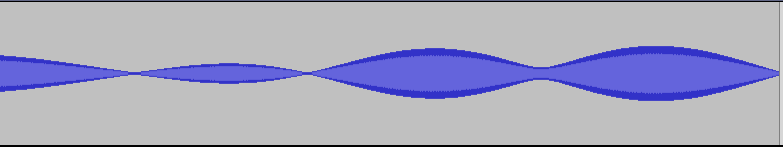
\includegraphics[width=1cm]{fadedsinesignal.png}
  \caption{Multi-path faded sine signal}
\end{figure}

Here is a GNU Octave or Matlab code for the used Rayleigh simulator which outputs a the signal as audio:
\begin{verbatim}
%Rayleigh simulator. Jakes model. In Octave remember to load the statistics package.

close all
clear all

tic

N = 20; %Number multipaths.
T = linspace(0,10000,100000); %Time.
v = 0.001; %Speed of the receiver.
randan = pi*rand(1,N); %Random angles w.r.t. receiver.
rI = 1000*rand(1,N); %Random distances of the sources.

%Geometrical stuff. Check for the Jakes model in the reference.
An = @(t) (atan(sin(randan).*rI./(cos(randan).*rI-v*t))).*(cos(randan).*rI>v*t)+...
(pi-atan(sin(randan).*rI./(v*t-cos(randan).*rI))).*(cos(randan).*rI<=v*t);
phis = 2*pi.*(rand(1,N));
wc =pi/2; %Frequency of the signal.
Beta = 2*pi/(1/(wc/(2*pi)));
theta = @(t) cos(An(t)).*Beta*v.*t+phis;

powers = rand(1,N); %Random powers of the signals in the multipaths.
powers = powers./sum(powers); %Normalize the powers.
Ez = @(t) sum(powers.*cos(wc*t+theta(t)));
EZ = []; %Faded signal.
REF = []; %Original signal.
NOISE = []; %Additional Gaussian noise.
for t =T
EZ = [EZ Ez(t)];
REF = [REF cos(wc*t)];
NOISE = [NOISE 0.9*stdnormal_rnd(1)];
end

%Write the audio files at sampling rate 8000.
audiowrite('EZ.wav',EZ,8000)
audiowrite('EZNOISE.wav',1/2*(EZ+NOISE),8000)
audiowrite('REFNOISE.wav', 1/2*(REF+NOISE), 8000)


toc
plot(T,EZ)
\end{verbatim}


And the same in Python:

\begin{verbatim}
  import numpy as np
  import math
  import matplotlib.pyplot as plt
  import sounddevice as sd
  import time

  #Jakes Rayleigh simulator. Please check for the reference in this site for further details.

  N = 20 #Number of multipaths.
  T = np.linspace(0, 10000, 100000) #Time vector.
  v = 0.001 #Speed of the receiver. 



  randan = np.random.rand(1, N) * math.pi #Random angles w.r.t. receiver.
  rI = np.random.rand(1, N) * 1000 #Random distances of the sources.
  phis = np.random.rand(1, N) * 2 * math.pi 

  def An(t):
  return (np.arctan(np.sin(randan) * rI / (np.cos(randan) * rI - v * t))) * (
  np.cos(randan) * rI > v * t
  ) + (np.pi - np.arctan(np.sin(randan) * rI / (v * t - np.cos(randan) * rI))) * (
  np.cos(randan) * rI <= v * t
  )

  wc = np.pi/2 #Frequency of the signal.
  Beta = 2 * math.pi / (1 / (wc / (2 * math.pi)))

def theta(t):
    return np.cos(An(t)) * Beta * v * t +phis

powers = np.random.rand(1,N)*2 #Random powers of the signals in the multipaths.
powers = powers/np.sum(powers) #Normalize powers..

def Ez(t):
    return np.sum(powers * np.cos(wc * t + theta(t)))

EZ = np.vectorize(Ez)(T)
REF = np.vectorize(lambda time : 2*np.cos(wc * time))(T)

#Play and plot.
fs = 8000
sd.play(EZ,fs,blocking = True)
#sd.play(REF,fs,blocking = True)
plt.plot(T, EZ)
plt.show()  
\end{verbatim}



References:
\begin{itemize}
\item William C. Jakes, ``Microwave Mobile Communications'', IEEE PRESS, 1974.
\end{itemize}



\subsection{June – Why Does MIMO Work?}

Multiple-input and multiple-output (\htmladdnormallink{MIMO}{https://en.wikipedia.org/wiki/MIMO}) antenna technology is used to exploit the \htmladdnormallink{multi-path propagation}{\ray} to improve the capacity of a communication link (i.e. more gigabytes of internet speed). In principle, capacity of the link can be increased merely by increasing the power of the transmitting antenna. However – apart from being energy-consuming – this increases also interference to any other receivers should they transmit in the same frequency band. In MIMO the energy is divided among multiple antennas, and the link capacity is improved without using any extra energy and without increasing the interference to other transmitters.

But what is the secret? Here is how I came up with a simple argument based on stochastic geometry.
Let us make some assumptions. We assume a flat and infinite Earth (yeah – you can laugh at this “tin foil assumption”, but it is often reasonable). In addition, we assume that our communication channel environment consists of many obstacles so that our transmitting antenna and receiving antenna can not see each other. We can assume that we are in a city full of houses, cars, trees, etc. Then our data signal is prone to propagate to the receiver through multiple paths; for example through distinct streets around different houses. The aggregate signal in the receiver will be  \htmladdnormallink{Rayleigh faded}{\ray}. The city is full of mobile phones exchanging data with their base stations which are further handing the data to the receiving mobile phones base station and, on the other hand, causing interference to the other base stations. We make a natural assumption that the interfering base stations are distributed according to the \htmladdnormallink{Poisson point process}{https://en.wikipedia.org/wiki/Poisson_point_process} around the receiver.

Let's consider that person A is sending a message (a Telegram message, or whatever you wish) to person B. We are interested in the probability that the base station serving person A will successfully transmit the message to a base station serving person B. Under assumptions above and some other simplified assumptions – as derived \htmladdnormallink{here}{\hall}, we can express the probability of a successful transmission as:

\begin{equation}
  \textbf{P}[\text{Successful single-antenna transmission}] = e^{-\frac{\pi^2}{2\sqrt{P}}},
\end{equation}

where $P$ denotes the mean transmitting power of the base-stations.

In MIMO we use multiple distinct antennas to transmit the same message. In each antenna, encoding of the message should be different so that it can't mix with the information that the other antennas are transmitting. This is possible by \htmladdnormallink{orthogonal modulation}{https://en.wikipedia.org/wiki/Orthogonal_frequency_division_multiplexing}.
Assuming that each message from each antenna will propagate to the receiver in an independent way, we can calculate from equation $(1)$ by complementary probability that \textbf{at least one message transmission gets through:}

\begin{equation*}
  \textbf{P}[\text{Successful MIMO transmission with N antennas}]  = 1-\left(1-e^{-\frac{\pi^2}{2\sqrt{P/N}}}\right)^N,
\end{equation*}

where $N$ is the number of transmitting antennas. Notice that we divided the transmitting power $P$ by the number of antennas, so we don't increase the aggregate power at all.
In the other hand, should we have no MIMO technology at hand, we could try to improve to increase the link quality just by increasing the power $P$ of a single antenna. In the following figure we compare these two cases.

\begin{figure}
  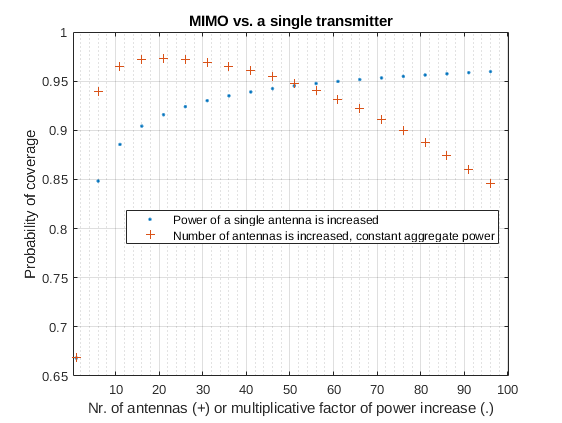
\includegraphics[width=\linewidth]{MIMO.png}
  \caption{MIMO saves energy and improves the quality}
\end{figure}

It is evident that MIMO is a great solution for increasing the throughput of a wireless communication link. Using multiple antennas we can save power and achieve better data-rates than by merely increasing the power of a single transmitter.

References:
\begin{itemize}
\item François Baccelli, Bartlomiej Blaszczyszyn \htmladdnormallink{Stochastic Geometry and Wireless Networks, Volume 2 - Applications}{\hall}
\end{itemize}

\subsection{July – Animating GIFs in GNU Octave}

Often it is nice to plot your results as an animation. The following code demonstrates the most effective way to write GIFs in Octave that I could find. Example code outputs an animation of a \htmladdnormallink{complex base-band signal symbol}{https://en.wikipedia.org/wiki/Quadrature_amplitude_modulation} in noise. Code uses the quiver plot, but any other plot should do equally well. Matlab compatibility is not guaranteed.

\begin{figure}
  \includegraphics[width=\linewidth]{gifu.gif}
  \caption{Animated GIF of a noisy QAM symbol}
\end{figure}


The point is to loop through all frames and save them to a file after each other with functions \textit{getframe} and \textit{imwrite}. 

\begin{verbatim}
function writeGIF()
  clear all;
  close all;
  clear imread;
  clear imwrite;
  
  N = 100; %%Number of frames.

  %%We use quiver plot as an example, but any other plot works equally.
  signal = 5 + 5*i; %%Baseband symbol.
  signal = signal + randn(1) + randn(1)*i ;   %%Add some Gaussian noise.
  quiver(0,0,real(signal), imag(signal))
  axis([[-10, 10],[-10, 10]])

  %%Write the first frame.
  frame = getframe(); %%Get the current frame.
  imwrite(frame.cdata,'gifu.gif','gif','writemode','overwrite',...
          'LoopCount',inf,'DelayTime',0.1);  %%Write the frame to gifu.gif and use delay time 0.1 seconds.
  
  for iii = 1 : N
    iii
    %%Write GIF.
    signal = 5 + 5*i; %%Baseband symbol.
    signal = signal  + rand(1) + randn(1)*i ;   %%Add some Gaussian noise.
    quiver(0,0,real(signal), imag(signal))
    axis([[-10, 10],[-10, 10]])
    
    frame = getframe(); %%Get the current frame.
    imwrite(frame.cdata, 'gifu.gif','gif','writemode','append','DelayTime',0.1); %%Write the frame to gifu.gif.
  end
end


\end{verbatim}

References: 
\begin{itemize}
\item \htmladdnormallink{Octave Image Processing}{https://octave.org/doc/v4.0.1/Loading-and-Saving-Images.html}
\end{itemize}


\subsection{August – Radio Waves in a Tunnel}


Everyone has some experience of how radio turns into static when one is driving into a tunnel. It just does not work (unless there is a special  \htmladdnormallink{radiating cable}{https://en.wikipedia.org/wiki/Leaky_feeder} installed inside the tunnel).
Once upon a night, I could not get sleep pondering on why does this happen. For example, water seems to behave differently; no matter how narrow the pipe, a water wave will go through it. Someone might have told me that \htmladdnormallink{FM}{https://en.wikipedia.org/wiki/FM_broadcast_band} radio wavelength is just so large that the wave “does not fit the tunnel”. But as intuitively acceptable as this explanation could be (I don't think it is even that), it is not a satisfying explanation as such.


After some research, I found that the explanation lies in the behaviour of \htmladdnormallink{Maxwell equations}{https://en.wikipedia.org/wiki/Maxwell's_equations} (well, what a surprise). All backs down to the boundary conditions of the electromagnetic field at the tunnel wall: the tangential component of the electric field component of the electromagnetic wave has to be near to zero in the tunnel interface. This leads to a situation where the wave has, in a sense, no room the oscillate inside the tunnel. The zero interface condition here is crucial; for example, it does not generally apply to a water wave and this is the reason a wave in the water fit through the smallest hole.


Intuitive or not, this is what the equations tell us. To demonstrate this fact I solved, using \htmladdnormallink{FEM}{https://en.wikipedia.org/wiki/Finite_element_method}, the \htmladdnormallink{Helmholtz equation}{https://en.wikipedia.org/wiki/Helmholtz_equation} for a plane-wave in a two-dimensional setting mimicking a tunnel and its entrance. The \htmladdnormallink{electromagnetic wave's}{https://en.wikipedia.org/wiki/Electromagnetic_radiation} polarization is so that the electrical component is pointing at the right angle w.r.t. the plane (either towards or against the reader of this page). \htmladdnormallink{Boundary conditions}{https://en.wikipedia.org/wiki/Boundary_value_problem} inside the 2D tunnel are zero. Solutions colouring shown in the figures following represents the magnitude of the electrical component.

We compare the behaviour of two different wavelengths:




\begin{figure}
  \includegraphics[width=\linewidth]{highfreq.gif}
  \caption{High frequencies fit in the tunnel}
\end{figure}


\begin{figure}
  \includegraphics[width=\linewidth]{lowfreq.gif}
  \caption{Wavelengths bigger than the diameter of the tunnel will not get through}
\end{figure}.



References: 
\begin{itemize}
\item \htmladdnormallink{Scattering Problem: Matlab PDE Modeler App}{https://se.mathworks.com/help/pde/ug/scattering-problem.html}
\item \htmladdnormallink{Interface conditions for electromagnetic fields (Wikipedia article)}{https://en.wikipedia.org/wiki/Interface_conditions_for_electromagnetic_fields}
\end{itemize}

  \subsection{September – The Universality of the Poisson Point Process (Breaking a Pile of Sand)}


  I thought that it would be nice to write about some purely mathematical subject today, so I decided to briefly discuss the famous Poisson process and its properties under a transformation.

  It is a well-known fact that some point processes converge to the Poisson point process after a sufficient amount of right transformations. This is of course why the Poisson p.p appears everywhere in nature; for example, grain of sands in a sand castle – made by a child at a beach on a sunny day – will eventually spread by wind (or water) around the beach. The grains will be randomly displaced here and there forming something approximating a realization of a Poisson p.p., even though the original pile was more ordered.

  Let's play the game with a pile of sand spreading to a flat area by random translations of the grains. 

  Consider a pile of sand at origo. Furthermore, let's assume that the pile is small enough (compared to unit distance) so that it is concentrated in a single point. Let's make a natural assumption that the amount of grains in the pile is  \htmladdnormallink{Poisson distributed}{https://en.wikipedia.org/wiki/Poisson_distribution}. Now our pile of sand is a Poisson point process concentrated in the origo.

  Suppose that after a while, wind moves individual sand grains from the pile directing them with a uniformly distributed angle and to a random normally distributed distance between $[0, \infty)$. In other words, the probability that a sand grain is moved from the origo to a location $Y_j$ inside a circle $B(r_1,r_2)$ is $2\int_{r_1}^{r^2} \frac{1}{\sqrt{2 \pi}}e^{-y^2} dy.$ 
  
  After a random translation of all points the \htmladdnormallink{Laplace functional}{https://en.wikipedia.org/wiki/Laplace_functional} of the \textit{distances} of the points is 

  \begin{align*}
    \mathcal{L}_{\tau}(f) &= \mathbb{E} \exp \left[-\sum_i f(|Y_i|) \right] = \mathbb{E}  \prod_i \exp \left[  -f(|Y_i|)   \right]  \\
    &= \mathbb{E}_n \left[  (2 \pi)^{-n/2}  \int_0^{\infty} \dots \int_0^{\infty}  \prod_{i = 0}^n \exp \left[  -f(y_i)  \right] \frac{2}{\sqrt{2 \pi}}e^{-y_i^2} dy_1 \dots d y_n \right] \\
    &= \mathbb{E}_n \left[(2 \pi)^{-n/2}  \left( \int_{0}^{\infty}  2\exp \left[  -f(y) - y^2   \right] dy \right)^n\right] \\
    &= \mathbb{E}_n \exp \left[ \sum_{i= 0}^n \log \left(   \int_{0}^{\infty}  \exp \left[  -f(y)  \right] \frac{2e^{-y^2}}{\sqrt{2 \pi}} dy \right) \right] \\ 
  \end{align*}

  Evaluating the  \htmladdnormallink{Poisson Laplace functional}{https://en.wikipedia.org/wiki/Poisson_point_process\#Laplace_functionals} $\mathcal{L}(g)$ of the sand pile with $ g = - \log \left(   \int_{0}^{\infty}  \exp \left[  -f(y)  \right] \frac{e^{-y^2}}{\sqrt{2 \pi}} dy \right)  $ we get
    \begin{align*}
      \mathcal{L}(g) = \mathcal{L}_{\tau}(f)& = \exp \left[  -\int_{\mathbb{R}^2} 1 -  e^{\log \left(   \int_{0}^{\infty}  \exp \left[  -f(y)   \right] \frac{2e^{-y^2}}{\sqrt{2 \pi}} dy \right) }\Lambda(dx) \right]    \\
      &= \exp \left[-\int_{\mathbb{R}^2} \left(1  -   \int_{0}^{\infty}  \exp [-f(y)] \frac{2e^{-y^2}}{\sqrt{2 \pi}}  dy \right)  \Lambda(dx)  \right] \\
        &= \exp \left[-\int_{\mathbb{R}^2}\int_{0}^{\infty} \left(1  -     \exp [-f(y)]   \right) \frac{2e^{-y^2}}{\sqrt{2 \pi}}dy  \Lambda(dx)  \right] \\ 
        &= \exp \left[-\int_{0}^{\infty} \left(1  -     \exp [-f(y)]   \right)  \sqrt{\frac{2}{\pi}}e^{-y^2} N dy    \right], (1) \\   
    \end{align*}

    where $N$ denotes the expected number of points in the sand pile (\htmladdnormallink{Campbell's theorem}{https://en.Wikipedia.org/wiki/Campbell\%27s_theorem_(probability)}). But the formula $(1)$ is the Laplace functional of the Poisson p.p. on $[0, \infty)$ with a density parameter $\sqrt{\frac{2}{\pi}}e^{-x^2} N.$  As the direction of the translation of a sand grain was uniformly distributed, we can conclude that the sand grains are Poisson distributed according to the Poisson p.p. with the two-dimensional multivariate Gaussian distribution as the density.
      
      The result above applies to any translations as long as the translation is independently applied to every point (or grain); the Poisson point process remains Poisson in a transformation. Here we had to make the Poisson assumption also for the pile so that the result above could be derived. But indeed, we can show that non-Poisson processes approach Poisson p.p. when the points are translated in a certain manner. However, I leave this is out of the scope of this blog entry for now, and take the remark made here as a simple (possibly a bit weird) example of the universality of the Poisson point process.
      
  \begin{figure}
    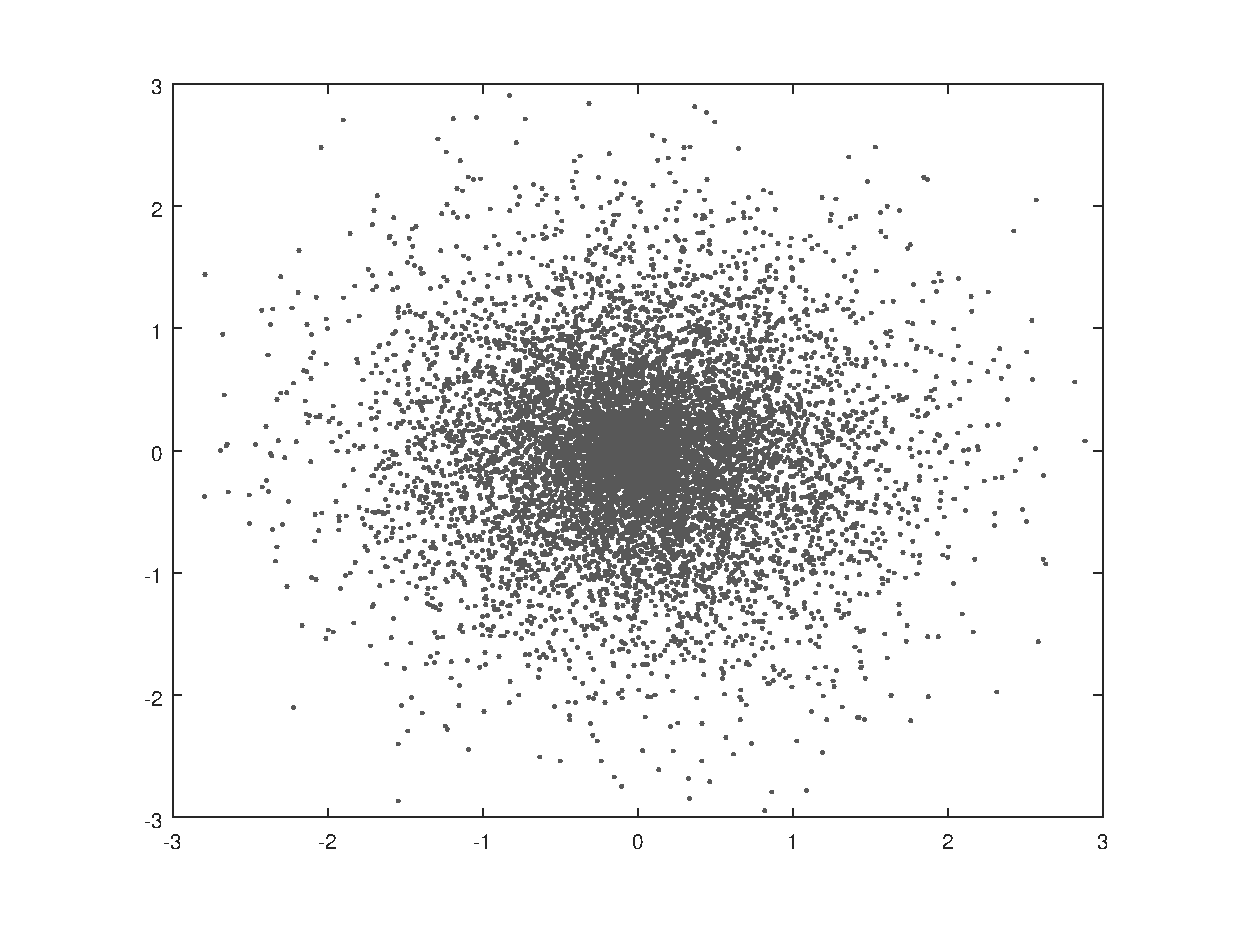
\includegraphics[width=\linewidth]{spread.eps}
    \caption{$10000$ points randomly moved from the origo to the plane}
  \end{figure}.


References:
\begin{itemize}
\item D. J. Daley and D. Vere-Jones, The General Poisson Process in  ``An introduction to the theory of point processes''. New York: Springer, Volume II: General Theory and Structure, 2008, pp. 166.   
\item François Baccelli, Bartlomiej Blaszczyszyn \htmladdnormallink{Stochastic Geometry and Wireless Networks, Volume I -Theory}{\hal}
\end{itemize}



\subsection{October – Fast Fourier Transform in GNU Octave}

\htmladdnormallink{Fast fourier transform}{https://en.wikipedia.org/wiki/Fast_Fourier_transform} (FFT) is an algorithm that computes the \htmladdnormallink{discrete Fourier transform}{https://en.wikipedia.org/wiki/Discrete_Fourier_transform}.

FFT is especially handy in real-time digital signal processing. Digital computers are working on discrete data, thus a input signal is always sampled with some sampling rate $F_s$ (Hz). By the \htmladdnormallink{Nyquist-Shannon sampling theorem}{https://en.wikipedia.org/wiki/Nyquist\%E2\%80\%93Shannon_sampling_theorem}, sampling captures frequencies under $F_s/2$.

Octave calculates the FFT of a discrete signal.  In the following code, we calculate the normalized FFT and plot the frequency spectrum w.r.t. the frequency. Signal vector and sampling frequency are given as input.

\begin{verbatim}
##Calculates the FFT and plots the frequency spectrum of a signal. Sampletimes have to start at time 0.

function fftvector = plotfft(signal, Fs)
  N = length(signal); #Signal length.
  FFT =  fft(signal);
  if(mod(N,2) == 0) #Check if signal length is odd or even.
    FFT = 2*FFT(1 : N/2)/N;
    f = Fs*(0 : (N - 1)/2)/(N - 1); 
  else
    FFT = 2*FFT(1 : (N - 1)/2)/N;
    f = Fs*(0 : (N - 2)/2)/(N - 1);
  end  
  fftvector = [f; FFT];
  
  figure(1)
  plot(f, abs(FFT));
  title('Fast fourier transform')
  xlabel('Frequency (Hz)')
  print  plot.jpg
end

\end{verbatim}

The following figure shows my track \htmladdnormallink{Tappimarssi}{https://soundcloud.com/ilari-angervuori/tappimarssi} in the frequency domain. The track was imported to Octave by

\begin{verbatim}
[signal, Fs] = audioread('Tappimarssi.wav');
\end{verbatim}



\begin{figure}
    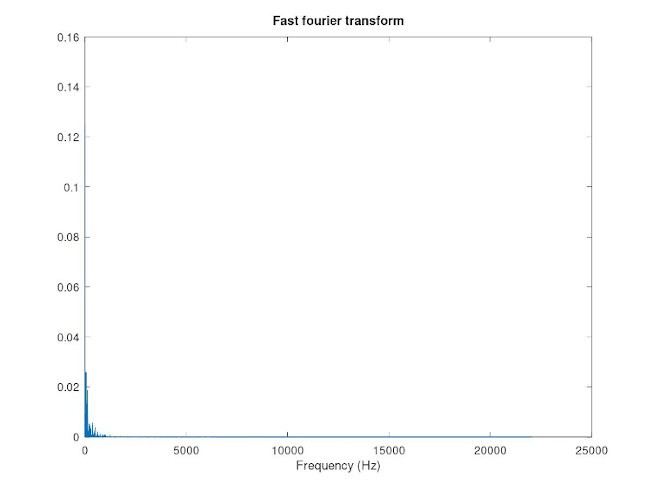
\includegraphics[width=\linewidth]{tappimarssi.jpg}
\end{figure}


\begin{itemize}
\item  \htmladdnormallink{Octave Documentation – Signal Processing}{https://octave.org/doc/v5.2.0/Signal-Processing.html}
\end{itemize}
  
\subsection{November – Digital Filtering}

Let's construct a simple digital band-pass filter based in the \htmladdnormallink{sinc filter}{https://en.wikipedia.org/wiki/Sinc_filter}.

As everyone know, the sinc function is the \htmladdnormallink{impulse response}{https://en.wikipedia.org/wiki/Impulse_response} of a low-pass filter. That is, the \htmladdnormallink{convolution}{https://en.wikipedia.org/wiki/Convolution} of a signal $ S(t)$ and the sinc function $ t \mapsto \frac{\sin(2 \pi B_L t)}{\pi t}$ will produce a low-pass filtered signal $S(t)$ without frequencies higher than $B_L$. Similarly, the function $ t \mapsto \delta(t) -  \frac{\sin(2 \pi B_H t)}{\pi t},$ where $ \delta(t)$ represents the \htmladdnormallink{Dirac delta function}{https://en.wikipedia.org/wiki/Dirac_delta_function}, is the frequency response of the ideal high-pass filter of frequency $B_H$.

Heuristically, we can right away derive the discrete versions of the impulse responses:

$$
\mathbb{Z} \ni i \mapsto \frac{\sin(2 \pi \frac{B_L}{f_c} i)}{\pi i},
$$
for the low-pass filter, and

$$
 i \mapsto \delta[i] - \frac{\sin(2 \pi \frac{B_H}{f_c} i)}{\pi i},
$$

for the high-pass filter. The variable $f_c$ is the sampling frequency and  $i \mapsto \delta[i] := \delta_{0i} $ is the \htmladdnormallink{Kronecker delta}{https://en.wikipedia.org/wiki/Kronecker_delta}.

Now, having a discrete signal at hand, band-pass filtering  is (in the simplest approach) just a matter of discrete convolution of the signal with the functions above. The following octave code does the job.


\begin{verbatim}
##Sinc band-pass filter. f0 = B_L/fs, f1 = B_H/fs

function filtered = sincfilter(signal, f0, f1)
  if(mod(length(signal), 2) != 0) #Check if the signal length is even or odd.
    signal = signal(1 : length(signal) - 1);
  end
  
  M = 10000; #Increase this to increase accuracy.
  sincF = zeros(1, M);
  for m =  -M/2 + 1 : 1 : M/2 
    if(!(m  == 0))
      sincF(m + M/2) = sin(2*pi*f1*m)./(pi*m);
    else
      sincF(m + M/2) = 2*f1;
    end
  end

  sincH = zeros(1,M);
  for m =  -M/2 + 1 : 1 : M/2 
    if(!(m  == 0))
      sincH(m + M/2) = -sin(2*pi*f0*m)./(pi*m);
    else
      sincH(m + M/2) = -2*f0 + 1;
    end
  end
  
  ##Plot stuff.
  figure(1)
  plot(sincF)
  figure(2)
  plot(signal)

  tic
  filtered = conv(signal, sincF, "same");
  filtered = conv(filtered, sincH, "same");
  toc

  figure(3)
  plot(filtered)
end


\end{verbatim}



\begin{figure}
  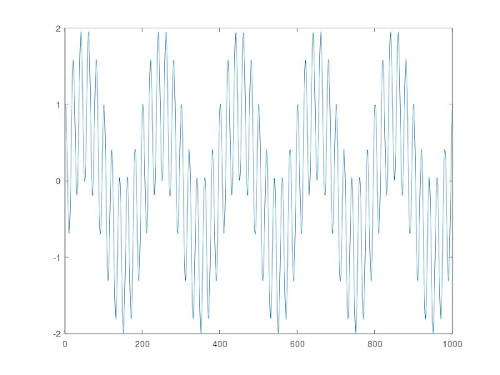
\includegraphics[width=\linewidth]{signal.jpg}
   \caption{Signal of form $\cos(20 \pi t) + \sin(2 \pi t)$}
\end{figure}

\begin{figure}
  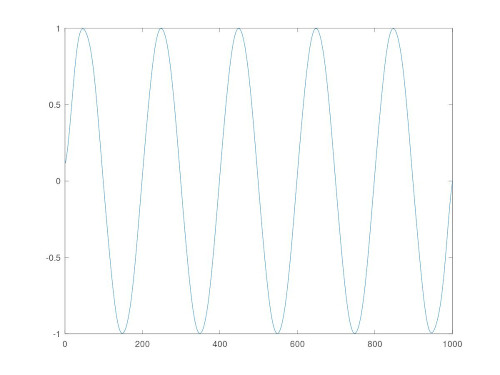
\includegraphics[width=\linewidth]{filtered.jpg}
   \caption{The same signal with the first term filtered away}
\end{figure}





For more accuracy and effectiveness, one should use windowed or recursive filters. You can check in the references for more sophisticated methods!


References:
\begin{itemize}
  \item Steven W. Smith, ``Digital Signal Processing – A Practical Guide for Engineers and Scientists'', Elsevier Science, 2003.
\end{itemize}


\subsection{December – Contour Plot in Mathematica}

A contour plot is a nice way to represent 2D data. Mathematica has great for constructing such plots, but you might want to tweak the fonts and graphics a bit. Sometimes fonts should be enlarged so that they are visible e.g. in a journal article where there is not too much space to use.

The following code returns a contour plot of the \htmladdnormallink{Riemann zeta function's}{https://en.wikipedia.org/wiki/Riemann_zeta_function} absolute value in an area in the complex plane; $(-2,10) \times(-10i, 10i) \subset \mathbb{C}.$ Text fonts are enlarged from default. Only values under $\max = 2$ are plotted. Values above that are ``clipped'' away as white colour. By definition of the absolute value, values are always more than $0$, otherwise values under $0$ would get clipped away with black colour. Contours are drawn in intervals of $0.1$, as adjusted in the \textbb{Range} function.
\begin{verbatim}
max = 2;
ContourPlot[Abs[N[Zeta[x + y*I]]], {x, -2, 10}, {y, -10, 10}, 
 PlotLegends -> BarLegend[{"Rainbow", {0, max}}], 
 ColorFunction -> "Rainbow", ContourStyle -> Black, 
 Contours -> Function[{min, max}, Range[min, max, 0.1]], 
 PlotLabel -> 
  Style["Absolute value of the Riemann zeta function", 16, Bold], 
 BaseStyle -> {FontSize -> 15}, 
 FrameLabel -> {Style["Real axis" , 16, Bold], 
   Style["Imaginary axis", 16, Bold]}, PlotRange -> {0, max}, 
 ClippingStyle -> {Black, White}]
\end{verbatim}


\begin{figure}
  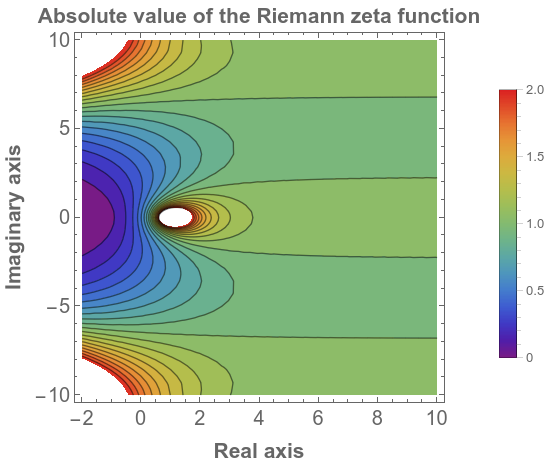
\includegraphics[width=\linewidth]{zeta.png}
\end{figure}



References:
\begin{itemize}
\item \htmladdnormallink{reference.wolfram.com}{https://reference.wolfram.com/language/guide/HypothesisTests.html}
\item Díaz-Francés, Eloísa; Rubio, Francisco J. (2012-01-24). "On the existence of a normal approximation to the distribution of the ratio of two independent normal random variables". Statistical Papers. Springer Science and Business Media LLC.
\end{itemize}


\section{Blog posts 2022}


\subsection{January – Inverse of a Gaussian Variable}

There is quite a pile of literature on the subject of the \htmladdnormallink{inverse}{https://en.wikipedia.org/wiki/Inverse_distribution} of a Gaussian distributed variable (this should not be fixed with inverse Gaussian distribution – it is a different matter). In fact, the inverse distribution is ill-behaved; the mean and variance does not generally exist.

I came up with a simple approximation that works well if the mean is large enough and the variance is small enough (I have not worked out the details of the exact conditions for this approximation. However, the results can be verified by Monte Carlo simulations). 

First, approximate the Gaussian distributed variable $X \sim \mathcal{N}(\mu, \sigma^2)$ by a log-normally distributed variable $X \approx Y \sim \text{Lognormal}(\mu_{\text{LN}}, \sigma_{\text{LN}}),$ with corresponding mean and variance, i.e.
$$\mu = \exp\left( \mu_{\text{LN}} + \frac{\sigma_{\text{LN}}^2}{2} \right)$$ and
$$\sigma = (\exp( \sigma_{\text{LN}}^2) - 1)\exp(2 \mu_{\text{LN}} + \sigma_{\text{LN}}^2).$$ We leave the solving of $\mu_{\text{LN}}$ and $\sigma_{\text{LN}}$ as an easy exercise for the reader.


Using the theory of log-normal distribution, the inverse of $X$ is now given by
$$
1/X \approx 1/Y \sim \text{Lognormal}(-\mu_{\text{LN}}, \sigma_{\text{LN}}).
$$

That's it!



References:
\begin{itemize}
\item \htmladdnormallink{Log-normal distribution}{https://en.wikipedia.org/wiki/Log-normal_distribution}
\item  Díaz-Francés, Eloísa; Rubio, Francisco J. (2012-01-24). "On the existence of a normal approximation to the distribution of the ratio of two independent normal random variables". Statistical Papers. Springer Science and Business Media LLC.
\end{itemize}


\subsection{February – Voronoi Tesselation on a Sphere}

Voronoi tessellation consists neighborhood areas of a given set of points, or Voronoi cells: every cell is surrounded by the area that consists of locations that are closer to the cell than any other cell. In addition to the artistic value, \htmladdnormallink{Voronoi Diagram}{https://en.wikipedia.org/wiki/Voronoi_diagram}, or Voronoi tessellation, have applications in wireless communications (among the million other things). 

\begin{figure}
  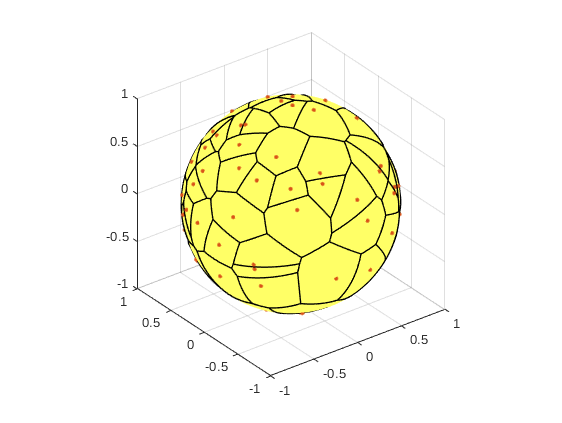
\includegraphics[width=\linewidth]{voronoionsphere.png}
\end{figure}


The next Matlab code produces a Voronoi tessellation on a sphere Poisson points as cells. It is based in Grady Wrights codes openly available in Github. 

\begin{verbatim}


%%Create Voronoi tesselation around Poisson points on a Sphere.

clear all;
close all;

addpath(fullfile(cd,'rbfsphere'));
density = 100;
X = poissononsphere(density)'; %Poisson points in spherical coordinates.
voronoiSph(X); %This function is downloaded from gradywright's Github. It is placed in the folder 'rbfsphere'.

function refc = poissononsphere(density)
  yMin = -1; yMax = 1;
  xMin = -pi; xMax = pi;
  
  xDelta = xMax - xMin; yDelta = yMax - yMin; %Rectangle dimensions
  numbPoints = poissrnd(density);    %Number of points in the area is a Poisson variable of intensity given as density
  x = xDelta*(rand(numbPoints,1)) + xMin;    %Pick points from uniform distribution
  y = yDelta*(rand(numbPoints,1)) + yMin;    %Map referencepoints to geographical coordinates
  ref = [x y]';

  refs = [x'; asin(y)'];%Map geographical coordinates to Cartesian coordinates on a unit circle
  r = 1;
  refc = [r*sin(refs(2,:)+pi/2).*cos(refs(1,:)+pi);...
          r*sin(refs(2,:)+pi/2).*sin(refs(1,:)+pi);...
          r*cos(refs(2,:)+pi/2)];
end

\end{verbatim}



References:
\begin{itemize}
\item \htmladdnormallink{gradywright Github}{https://github.com/gradywright/spherepts/tree/master/code}
\end{itemize}



\subsection{March – Plotting in Mathematica}

Here's a plot for Mathematica that you can use as a template to plot ListLinePlot and Plot in the same figure. Font sizes are increased to be well visible in a research article. 


\begin{verbatim}
xmax = 150;
ymax = 0.025;
Show[
 (*Histogram[res1,Automatic,"PDF"],*)
 
 ListLinePlot[{Table[{t, 
     PDF[GammaDistribution[3.715287738432738`, 16.575007504627795`]][
      t]}, {t, 0, xmax, xmax/10}],
   Table[{t, 
     PDF[GammaDistribution[6.502676225156808`, 8.60919186301341`]][
      t]}, {t, 0, xmax, xmax/10}], 
   Table[{t, 
     PDF[GammaDistribution[3.3444580518527207`, 16.73897127052263`]][
      t]}, {t, 0, xmax, xmax/10}]}, 
  PlotRange -> {{0, xmax}, {0, ymax}},
  PlotLabel -> PDF,
  AxesLabel -> {Style["SIR", 16, Bold], Style["", 16, Bold]}, 
  PlotLegends -> Placed[{"Sim 1", "Sim 2", "Sim 3"}, Right], 
  PlotMarkers -> {Automatic, 10}, BaseStyle -> {FontSize -> 15}],
 Plot[
  {
   PDF[GammaDistribution[3.715287738432738`, 16.575007504627795`]][
    t],
   PDF[GammaDistribution[6.502676225156808`, 8.60919186301341`]][t],
   PDF[GammaDistribution[3.3444580518527207`, 16.73897127052263`]][t]
   }, {t, 0.01, xmax}, PlotStyle -> Thick, 
  PlotLegends -> 
   Placed[{"\[CapitalGamma](3.7, 16.6)", "\[CapitalGamma](6.5, 8.6)", 
     "\[CapitalGamma](3.3, 16.7)"}, Right]]
 ]
\end{verbatim}


Output:
\begin{figure}
  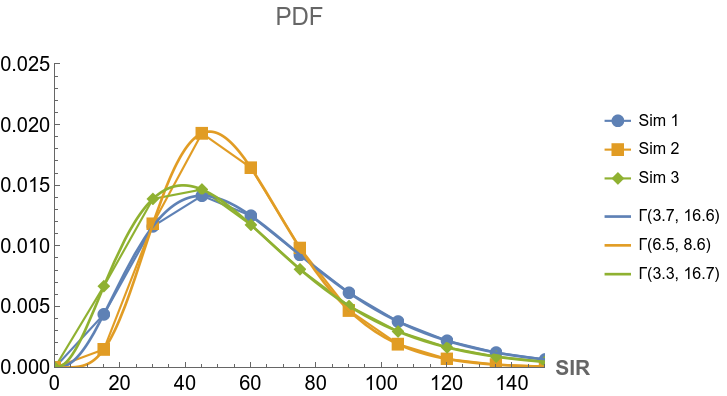
\includegraphics[width=\linewidth]{listlineplot.png}
\end{figure}


References:
\begin{itemize}
\item \htmladdnormallink{reference.wolfram.com}{https://reference.wolfram.com/language/guide/HypothesisTests.html}
\end{itemize}


\subsection{April – Satellite Communication Toolbox in Matlab}

Matlab's Satellite Communication Toolbox can be used to study and visualize satellite networks. The following code places a terrestrial station in Otaniemi, and a LEO satellite in $2000$ km tracking the station. Satellite have to be at least in a elevation angle of $35$ degrees to contact to the base station. Satellites field of view and a $3$ dB footprint of width $1.5$ degrees is also represented.

\begin{verbatim}
clear all;
close all;

startTime = datetime(2020,8,19,20,55,0); % 19 August 2020 8:55 PM UTC
stopTime = startTime + days(1);          % 20 August 2020 8:55 PM UTC
sampleTime = 60;                         % seconds
sc = satelliteScenario(startTime,stopTime,sampleTime);


semiMajorAxis = (6378 + 2000)*1000;          % meters
eccentricity = 0;
inclination = 90;                   % degrees
rightAscensionOfAscendingNode = 0; % degrees
argumentOfPeriapsis = 0;           % degrees
trueAnomaly = 0;                   % degrees
sat1 = satellite(sc, ...
    semiMajorAxis, ...
    eccentricity, ...
    inclination, ...
    rightAscensionOfAscendingNode, ...
    argumentOfPeriapsis, ...
    trueAnomaly, ...
                 "Name","Satellite", ...
                 "OrbitPropagator","two-body-keplerian");

sat1.LabelFontSize = 30;
cam1 = conicalSensor(sat1,"MaxViewAngle",90)
cam2 = conicalSensor(sat1,"MaxViewAngle",1.5/2)

name = "Test Transmitter";
minElevationAngle = 35; % degrees
lat = 60.185;
lon = 24.83;
geoSite = groundStation(sc, lat, lon, "Name", name, "MinElevationAngle", minElevationAngle)
geoSite.LabelFontSize = 30;
ac1 = access(cam1,geoSite);
ac2 = access(cam2,geoSite);

fov1 = fieldOfView(cam1, "LineColor",'blue', "LineWidth", 10)
ac1.LineColor = 'black';

fov2 = fieldOfView(cam2, "LineColor", 'green', "LineWidth", 10)

pointAt(sat1,geoSite);

play(sc);

\end{verbatim}



Output:
\begin{figure}
  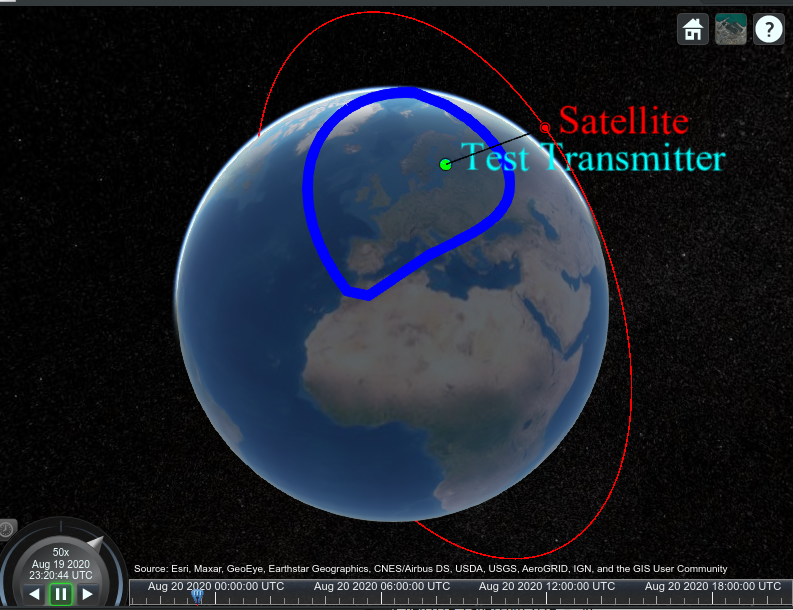
\includegraphics[width=\linewidth]{stk.png}
\end{figure}


References:
\begin{itemize}
\item \htmladdnormallink{Mathworks}{https://se.mathworks.com/products/satellite-communications.html}
\end{itemize}



%\subsection{December – Quadrature Amplitude Modulation}



\end{document}
%
% optional post-title formatting for PostScript
%
\parindent0pt
\parskip2.5ex plus 0.5ex minus 0.5ex

